\cleardoublepage
\chapter{Arquitectura y diseño.}
\label{chap:design_implement}

En este capítulo, vamos a describir la metodología de desarrollo del proyecto Misture, y el diseño y arquitectura en varios momentos de su desarrollo, respondiendo a una funcionalidad creciente y más rica.\\


Por último, se detalla de forma lo más aproximada posible la estructura de la base de datos no relacional que se emplea en el estado final del proyecto.\\


\section{Modelo de desarrollo} 
\label{subsec:modelo_desarrollo}

El desarrollo de un proyecto de software libre implica una sucesión de tareas entre el momento que se tiene una idea para resolver un problema o necesidad, y el producto u servicio final que lo satisface. Este metodología nos marca como se suceden las diferentes tareas y actividades dentro del proyecto.


Durante el desarrollo de este proyecto hemos seguido un modelo que se asemeja al modelo de desarrollo iterativo y creciente, o incremental. En este proceso creamos una primera versión del sistema que sea funcional, con el que se pueda interactuar y nos proporcione realimentación para las sucesivas iteraciones. \newpage	%TODO AJUSTE




El modelo incremental, a priori, nos proporciona las siguientes ventajas:

\begin{itemize}
\item Al desarrollar sistemas más pequeños con subconjuntos de los requerimientos o funcionalidades, reducimos el riesgo asociado a realizar el desarrollo en bloque del sistema completo.

\item Al desarrollarse progresivamente parte de las funcionalidades, se puede evaluar mejor si los requerimientos de los siguientes incrementos son correctos o hay que adaptarlos a la realidad.

\item En caso de errores o problemas, generalmente afectan a la última interacción y no a todo el conjunto, volviendo al incremento previo en el peor caso.

\item En el caso de este proyecto, permitía avanzar paso a paso en el desarrollo del sistema mientras se iba adquiriendo la experiencia necesaria para desarrollar mejor o redefinir mejor los siguientes incrementos.
\end{itemize}


Además, este modelo tiene gran similitud con el modelo que nuestro profesor adoptaba para la evolución de las prácticas de sus asignaturas durante el curso. Estas empezaban con prácticas sencillas o introductorias, a las que se le iban añadiendo elementos, funcionalidades y complejidad hasta llegar a la práctica final, que en realidad era una sucesión de incrementos a partir de una estructura inicial que se había establecido prácticas atrás.


Para observar esto último, en el caso de este proyecto, disponíamos de algunas muestras de grupos de repositorios de las actividades en diferentes etapas del trimestre los cuales, por ejemplo, podemos clasificar según a la exigencia que nos va a suponer para nuestro sistema corrector Misture. \newpage	%TODO AJUSTE




\textbf{GRUPO 1}


\begin{itemize}
\item Actividades en las semanas iniciales del trimestre o introductorias.

\item Pequeños proyectos con poca cantidad de código y elementos que exige un análisis de código Python más simple.

\item Salidas de ejecuciones más sencillas: cierto fichero con un contenido concreto, cadenas cortas de valores concretos, etc.

\item Puede requerir algunas comprobaciones sencillas sobre ficheros o documentos XML

\item Por el momento, al alumno se le está introduciendo en temas de calidad y estilo de código y es suficiente contar los errores e imprimirle al alumno qué errores comete, qué significan y en qué código se produce.
\end{itemize}

\vspace{1cm}
\textbf{GRUPO 2:}


\begin{itemize}
\item Actividades de etapas avanzadas del trimestre o de materias de mayor nivel.

\item Escenarios de mayor cantidad y complejidad de código fuente: aplicaciones cliente-servidor con lógicas complejas, desarrollo de aplicaciones sobre frameworks que conllevan mayor complejidad en la estructura del proyecto entregado, etc.

\item Análisis de código Python más complejo y rico.

\item La propia prueba de ejecución de la aplicación o aplicaciones se vuelve más difícil, y no nos sirven de igual forma cierto tipo de pruebas de ejecución en unos escenarios u otros.

\item En este punto, es interesante obtener información más rica sobre estilo y calidad de código y errores, para poder luego analizarse o reportarse asociado a su fichero fuente, u observar la evolución temporal de la calidad y errores de nuestro código.
\end{itemize}


De acuerdo al modelo de desarrollo descrito, en una fase inicial recogimos de forma general los requerimientos del sistema completo en base a la descripción del problema y las experiencias previas descritas en el Capítulo \ref{chap:objetivos} de la presente memoria.


Una vez se disponen de los requisitos, se crea una versión inicial funcional, que comenzamos con un modulo principal que dispone de las configuraciones básicas para obtener los repositorios y conocer los requisitos básicos como qué ficheros deben entregarse.


A partir de ese versión inicial, se fueron añadiendo los módulos con los diferentes grupos de funcionalidades, los cuáles íbamos probando frente a las muestras de los repositorios de alumnos. Es decir, realizábamos un incremento para agregar funcionalidad básica de análisis de código Python, posteriormente otra iteración para la extracción de información básica del repositorio Git, etc.


Entre dos incrementos, las únicas entradas de las que disponemos son los requisitos y el resultado de la interacción entre el cliente y el resultado del incremento anterior. En este caso el cliente somos nosotros probando los repositorios de las actividades de los alumnos.


Para simplificar la explicación del diseño de Misture, vamos a reducir la explicación de todo el proceso al detalle de dos estados, que vamos a denominar iteración 1 e iteración 2, que realmente componen una sucesión de incrementos que llevaron a esos dos estados del proyecto.


Esta división, asimismo, tiene también como justificación el hecho de que el estado descrito en la primera iteración es más próxima a las actividades caracterizadas del grupo 1 descrito anteriormente, y la iteración 2 recoge un estado más cercano a resolver las necesidades de las actividades descritas en el grupo 2.

\section{Iteración 1:}

Vamos a describir el diseño de los diferentes módulos que componen este primera sucesión de incrementos. En la figura de abajo se muestra un esquema de flujo de está primera versión de Misture.


En este diseño, para el almacenamiento y tratamiento de todos los datos extraídos en los diferentes análisis, se emplearon ficheros en las transacciones con las utilidades externas y para generar logs de errores e imprimir el reporte final ordenado. También se utilizaron estructuras dinámicas como listas, diccionarios y una jerarquía de clases Python que modelaban los diferentes objetos y las relaciones entre ellos que identificábamos en este escenario, tales como actividad, alumnos, repositorios, ficheros, elementos de código, estadística, error de estilo, etc.


Esta jerarquía de clases, es una primera versión del modelo de datos que será usado en la iteración 2 y que se detallará posteriormente en el apartado DISEÑO DE BBDD.



\begin{figure}[H]
   \centering
   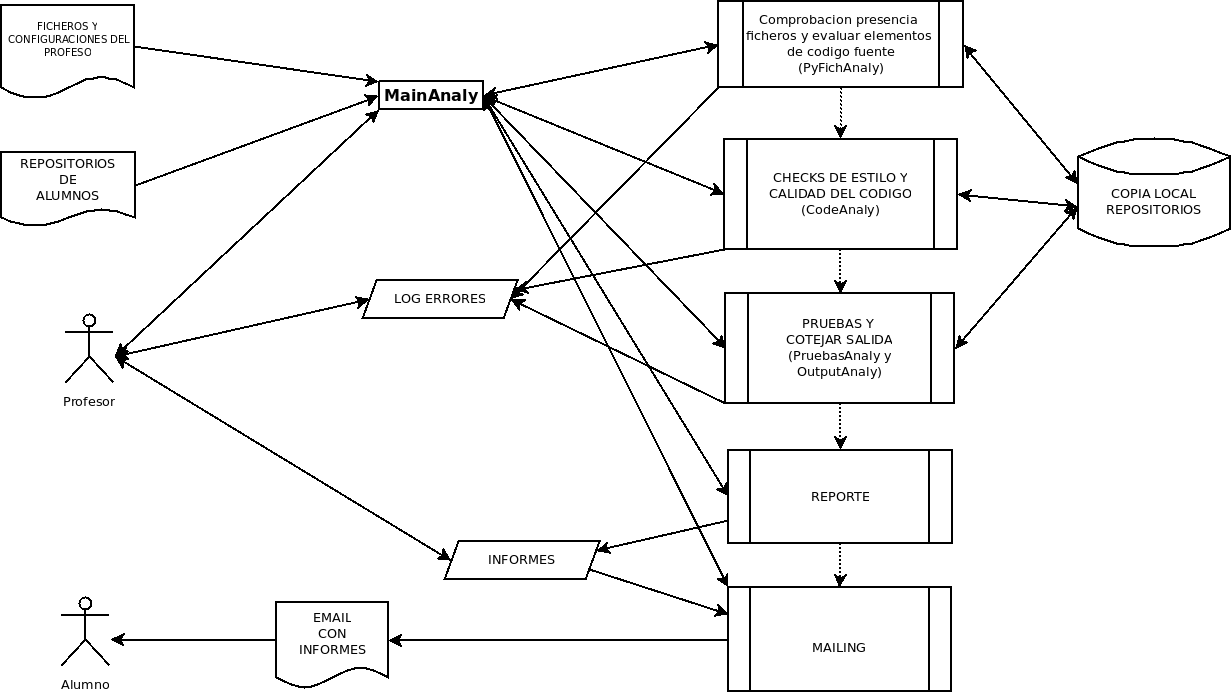
\includegraphics[width=12cm]{img/Diagram2_iteracion1}
   \caption{Flujo de la iteración 1.}
   \label{figura:ite1}
\end{figure}


\subsection{Módulo principal}

En el modulo \textit{MainAnaly}, se establece la configuración básica de la actividad a corregir, como la ubicación de los repositorios asociados a los logines de alumnos, los nombres de los ficheros y códigos fuentes que deben estar en el repositorio. Así como las tuplas con las llamadas a los programas del alumno, y las salidas que debe obtener el programa en caso de funcionar correctamente según la especificación de la actividad.


Este módulo, también se encarga de cargar esta configuración en la jerarquía de clases del escenario, inicializar los logs para la actividad, y establecer una ubicación para los reportes individualizados.


A continuación, se realiza las diferentes llamadas a los módulos de análisis, a los que se les proporciona como parámetros los objetos adecuados del escenario -repositorio, fichero, etc- y se recoge los resultados del análisis, asociándolos al objeto del mundo Misture correspondiente.

Al final del flujo se invoca a los objetos Misture para que se vuelque su información ordenada a los ficheros de reporte del alumno asociado, y se ordena al módulo de comunicación enviar en lote todos los reportes a los alumnos.

\subsection{Módulo de análisis de código Python}

Este módulo, llamado \textit{PyfichAnaly}, implementa la funcionalidad relativa a la identificación de los ficheros presentes en el repositorio del proyecto, en función de una lista definida de ficheros que se esperan de los alumnos.


Como novedad, en este análisis se detecta si al alumno le falta alguno de los ficheros requeridos por la práctica, y a través de una pequeña heurística intenta deducir si hay otros ficheros que de nombre similar que puedan serlo.


Esta heurística, se basa en el algoritmo de Levenhstein. Este algoritmo tiene la capacidad de medir la cantidad de operaciones de inserción, borrado o cambio de caracteres que hay entre dos cadenas de texto.


Por tanto, en caso de que se encuentren archivos huérfanos en la lista de ficheros requeridos y en el repositorio, y siempre que no supere un umbral, se entiende que el fichero con la menor distancia de Levenhstein es aquel que nos falta, y por tanto, se renombra y se prosiguen los análisis.


Una vez identificados los ficheros disponibles, se identifican los que son ficheros fuente Python, y se llama a la clase \textit{PyModuleCont}, que analiza el código fuente del fichero a través de patrones regulares y funciones de las librería \textit{re} de Python, cuya muestra se adjunta en la figura inferior.


De dicho análisis, asociamos al fichero Python los elementos clase, método y función que contengan, junto a su nombres.


\begin{figure}[H]
   \centering
   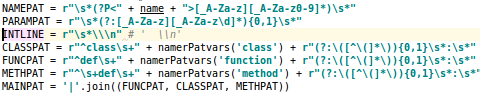
\includegraphics[width=16cm]{img/Selection_022_pyanaly_regex}
   \caption{Patrones utilizados para identificar elementos de código y su nombre}
   \label{figura:regex}
\end{figure}

\subsection{Módulo de análisis de calidad de código}

En el módulo \textit{CodeAnaly}, se implementa la funcionalidad de análisis de calidad del código, que en esta iteración del desarrollo de Misture, se realiza con ayuda de las utilidades \textit{Pep8}, para el análisis de estilo, y \textit{Pylint}, para el análisis estático del código.


El procedimiento de análisis de estilo, se implementa en la clase \textit{Pep8Analy}, es una clase con los atributos necesarios para almacenar los errores de estilo, ficheros en que se producen, y estadísticas de los errores.


\textit{Pep8Analy}  recibe como configuración las rutas de los ficheros Python a analizar, y los códigos de error que no deben ser tenidos en cuenta para este análisis. Y se inicializa invocando a la utilidad \textit{Pep8} como se indica abajo, para recopilar los errores detectados y un sumario de estadísticas.

\begin{center}
\begin{verbatim}
$ pep8 --repeat --show-source –ignore=<cods_error> <rutas_py>
$ pep8 -q --statistics <rutas_py>
\end{verbatim}
\end{center}


Por otra parte, también se implementa una clase \textit{PylintAnaly}, que con un funcionamiento semejante al de \textit{Pep8Analy}, extrae y guarda de forma estructurada los errores \textit{Pylint} y la nota de calidad del código obtenidas de la utilidad llamada de la siguiente manera.

\begin{center}
\begin{verbatim}
$ pylint --disable=<codigos_error> <ruta_py1 ruta_py2 ...>
\end{verbatim}
\end{center}


\subsection{Módulo de pruebas de ejecución}

A través del módulo \textit{PruebasAnaly}, en esta versión de Misture se ejecutan y almacenan los resultados para ser asociados a la corrección del alumno, una batería de pruebas que debe ser proporcionada al ser invocado la interfaz del test, implementado en la clase \textit{testPr} del módulo.

Cada elemento de la batería de pruebas es una prueba simple a través de una llamada a uno de los programas o scripts del alumno, sobre la ruta de su repositorio. Cada prueba, esta representada por una 3-tupla de etiqueta, prueba a ejecutar, y un tercer elemento que es una tupla con el contenido de las líneas que debemos recoger a la salida estándar de la prueba para dar por válida la prueba.


\begin{figure}[H]
   \centering
   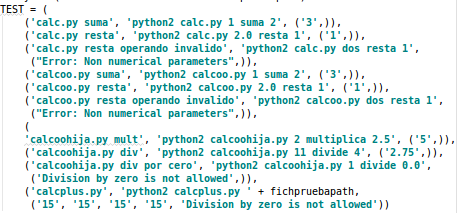
\includegraphics[width=16cm]{img/Selection_024_testcodigo}
   \caption{Tuplas con la batería de pruebas}
   \label{figura:testcodigo}
\end{figure}

La clase \textit{testPr} itera sobre cada una de las tuplas de prueba, ejecuta la prueba, e invoca a un pequeño módulo denominado \textit{OutputAnaly}, que chequea a través de funciones de texto y de la librería \textit{re} de Python que la salida recogida es compatible con la salida esperada, permitiendo cierta incertidumbre introducida por cambios en la capitalización, introducción de separadores o caracteres blancos, etc.

\subsection{Módulo de análisis de GIT}


En esta versión de Misture, se implementa un análisis sencillo de repositorio Git. Dicho análisis, se realiza a través del parseo de la salida de la siguiente llamada a Git.
\begin{center}
\begin{verbatim}
$ git log <ruta_repo_alumno>
\end{verbatim}
\end{center}

A la salida del \textit{log}, se le extraen mediante funciones de la librería \textit{re} de Python y los patrones adecuados los datos del autor del \textit{commit}.


Asimismo, podemos proporcionarle un listado de palabras o raíces de palabras que consideramos clave en los \textit{commits} de la actividad que corregimos por su significancia, obteniendo  del análisis el número de apariciones, y en consecuencia, una medida sobre si el alumno etiqueta los \textit{commits} con buen criterio.

\newpage	%TODO AJUSTE

\begin{figure}[H]
   \centering
   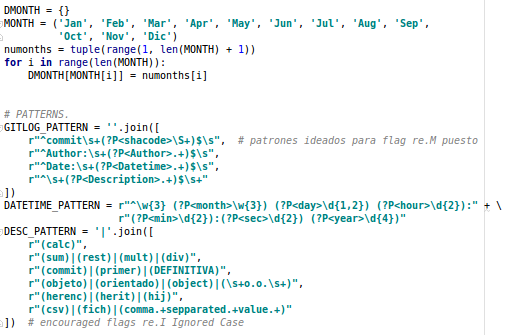
\includegraphics[width=16cm]{img/Selection_025_gitlog_patterns}
   \caption{Regex utilizados para el análisis del log}
   \label{figura:reg_analisis_log}
\end{figure}

\subsection{Módulo de comunicación}

Con el objetivo de dotar de nuevas funcionalidades a Misture y automatizando y reduciendo el tiempo necesario para todas las tareas. Se implementó una funcionalidad con el objetivo de poder comunicar masivamente el resultado de las prácticas. Esta funcionalidad la implementamos en el módulo \textit{mailing}.

En dicho módulo, a través la funcionalidad de las librerías \textit{smtplib} y \textit{email} de Python, o la API del servicio de emailing \textit{SendGrid}, hay implementaciones para realizar el envío automatizado de los reportes, siempre y cuando se proporcionen las credenciales de acceso.	\newpage %TODO AJUSTE

\section{Iteración 2:} 
\label{subsec:iteracion2}

Una vez descrito el diseño y funcionalidad de Misture en el estado anterior, podemos observar que el diseño propuesto en ese punto, introduce algunas pequeñas mejoras en cuanto a funcionalidades, organización y modularidad del sistema, especializando las tareas y diferentes tipos de análisis .


Asimismo, se ha establecido un universo de objetos que modela aproximadamente los elementos que nos vamos encontrando en una corrección automática y la generación de resultados de \textit{checks}, y así disponer de toda la información extraída en los análisis de una forma estructurada.


De esta forma, se facilita la recuperación de la información, pudiéndose elaborar diferentes informes al final del proceso corrección partiendo de la misma estructura de información, en lugar de componer una combinación heterogénea y por separado para alumno y profesor de trazas de diferentes ficheros sobre la marcha. También se facilita la posibilidad de añadir con más facilidad en pasos posteriores del proceso, otros análisis a partir de la información estructurada de la corrección. Por ejemplo, para añadir un pequeño análisis de la actividad a nivel de grupo, mediante la agregación de la información sobre cualquiera de los análisis.


Aun así, a pesar del trabajo desempeñado, la funcionalidad no supone una mejora cualitativa con respecto al sistema de \textit{scritps} de preproceso y corrección que se plantea en las experiencias piloto de los que partimos. Además, seguimos circunscritos a la corrección de entregas de tamaño reducido, con un pull de ficheros cerrado, y comprobaciones basadas en el parseo de la salida de trazas de terceras utilidades.


Por tanto, esta aproximación, una vez nos planteamos ampliar la funcionalidad, añadir más información para cada uno de los análisis, y trasladarlo a las correcciones de entregas más complejas y avanzadas, nos damos cuenta que es algo limitada para tales intenciones.


Tras recapitular estas ideas, es posible vislumbrar qué líneas vamos a seguir en la mejora del proceso. Por tanto, en los sucesivos incrementos de funcionalidades, se buscaron las siguientes mejoras:

\begin{itemize}
\item Estructurar la información en BBDD

\item Especializar aún más los módulos de análisis.

\item Búsqueda de APIs Python de las utilidades que se emplean para el análisis, o de alternativas que nos ayuden a tal fin.
\end{itemize}

A raíz de los cambios introducidos en el diseño de los sucesivos incrementos que realizamos en esta segunda versión de Misture, la estructura del código resultante se amplió, constando el proyecto con la siguiente estructura:

\begin{itemize}
\item El \textit{script} o módulo principal, desde el que se deben especificar las configuraciones y entradas -listados, ruta de ficheros del profesor, etc- necesarias para la corrección, y se invocan las llamadas a los análisis disponibles con los parámetros que el profesor quiera lanzar.

\item Un paquete de entidades –denominado \textit{entities}- donde se representan a los objetos del universo Misture, mapeados como documentos a una BBDD MongoDB.

\item Un paquete que contiene todos los módulos especializados que proporcionan acceso a cada pequeña funcionalidad de análisis implementada a través de, denominado \textit{Analyx}.

\item Se añade un paquete, cuya función consiste en hacer de intermediario entre los tres elementos anteriores, denominado \textit{funcionalityx}. Proporciona al módulo principal la interfaz sobre las funcionalidades de análisis a usar. Después, para cada funcionalidad, se encarga de invocar las operaciones y análisis especializados necesarios de los módulos del paquete \textit{analyx}. Y por último, es el encargado de interaccionar con las entidades del paquete \textit{entities}, de forma que la información que recibe de los análisis la almacene estructurada en los objetos del ODM, que se almacenaran de forma persistente en la BBDD.
\end{itemize}

A continuación, se describen dichos paquetes.

\begin{figure}[H]
   \centering
   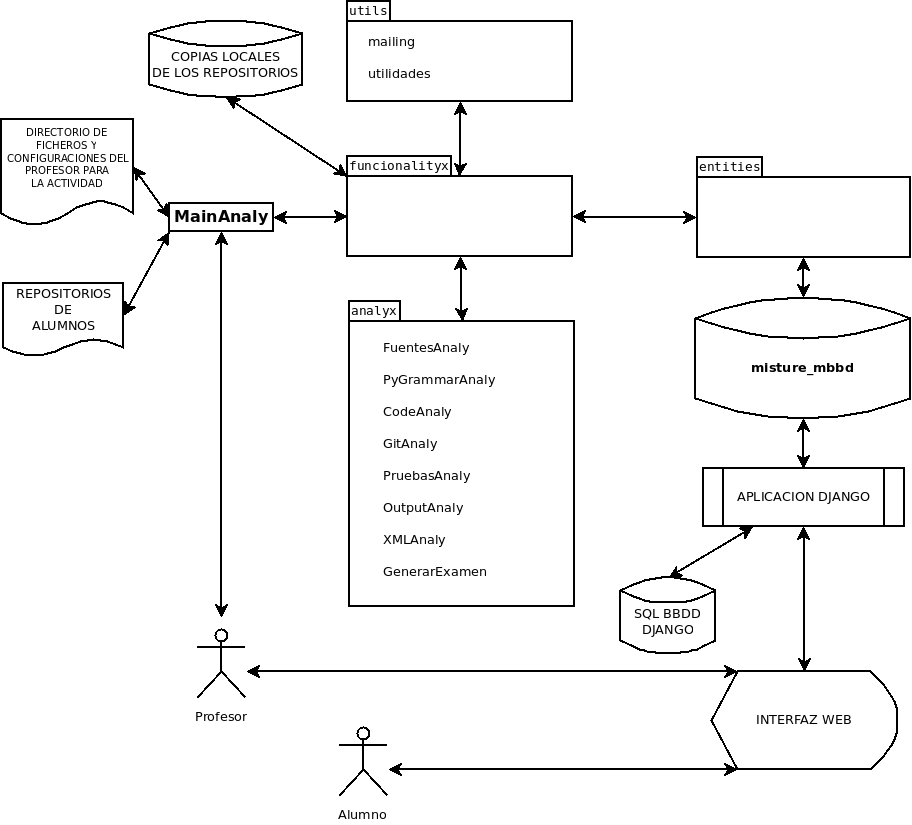
\includegraphics[width=16cm]{img/Diagram3_iteracion2}
   \caption{Relación entre los paquetes y elementos en esta versión de Misture}
   \label{figura:regex}
\end{figure}



\subsection{Módulo principal} 
\label{subsec:mod_principal}

Durante el transcurso de las iteraciones, se sigue manteniendo en el diseño el módulo principal como elemento de interacción con el profesor para la configuración, control y uso de la funcionalidad de Misture. La idea es que este módulo abstraiga el resto del sistema Misture y únicamente pueda usarse con la interfaz que proporcionemos a través del paquete \textit{funcionalityx}, siendo sólo necesario editar la configuración y llamadas a los análisis deseados para realizar cualquier corrección.


Se mantiene la necesidad de disponer de los listados de alumnos y de la ubicación o url de los repositorios, así como de las tuplas con las pruebas de caja negra a ejecutar. Además, se introduce como novedad la definición en la configuración de un directorio del profesor especifico para cada corrección, donde se depositan los ficheros externos necesarios para las funcionalidades como las preguntas de examen, ficheros de entrada u otros módulos, por ejemplo la implementación de un cliente o servidor para usarlo en las pruebas contra la implementación de los alumnos.

\subsection{Paquete de entidades} 
\label{subsec:paq_entities}

En la primera versión de Misture, se implementó una pequeña jerarquía de clases, con relaciones entre sí, que modelaban las diferentes realidades dentro de la corrección, con sus datos y relaciones entre ellos: una actividad, una corrección de actividad sobre un repositorio, un error de estilo o código, etc.


El siguiente paso en el diseño, ha sido trasladar este modelado a BBDD, de forma que podamos almacenar y recuperar sistemáticamente la información, y disponer de toda la información para posteriores reportes o análisis.


Al establecer el diseño de este paso, se optó por una base de datos no relacional como MongoDB, ya que para nuestro desarrollo incremental era más ágil y menos problemático no tener la exigencia de cumplir con un esquema fijo en los datos en todo momento.


Por otra parte, para poder centrarnos en la lógica de negocio de Misture, y abstraernos lo máximo posible de los accesos a datos, optamos también por el uso de un ODM, eligiendo \textit{PyMODM}. De esta forma, podemos mantener la lógica de nuestro universo de objetos Misture y ampliarla con mayor facilidad.


Asimismo, \textit{PyMODM} nos permite establecer el tipo de sus campos y otras restricciones, además de implementar validaciones como vemos en las figuras. Estas siempre se realizan a nivel de aplicación y no en BBDD.


\begin{figure}[H]
   \centering
   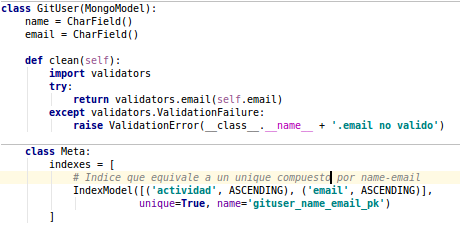
\includegraphics[width=16cm]{img/Selection_026_mongomodel}
   \caption{Un objeto Misture como documentos de una colección en MongoDB vía ODM}
   \label{figura:iter2}
\end{figure}

\begin{figure}[H]
   \centering
   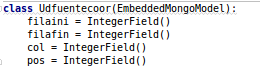
\includegraphics[width=8cm]{img/Selection_027_mongoembdoc}
   \caption{Representación de un documento sin colección, embebido en otro documento}
   \label{figura:mon_emb}
\end{figure}


\subsection{Paquete de funcionalidades} 
\label{subsec:paq_functs}

Como ya se ha introducido, este paquete \textit{funtionalityx} se encarga de implementar las funcionalidades de Misture a alto nivel, delegando las diferentes tareas que conforman un análisis a los módulos especializados del paquete \textit{analyx}, estructurando los datos recibidos en los objetos del ODM para su guardado en las colecciones de MongoDB, y atendiendo a las llamadas que recibe de la interfaz que sirve al módulo principal.


Las funcionalidades que podemos invocar, son las que se detallan a continuación.

\begin{itemize}
\item Análisis de ficheros del repositorio.

\item Análisis de elementos del código Python.

\item Análisis de estilo y calidad del código.

\item Análisis de repositorio Git.

\item Análisis de XML y trazas de Wireshark.

\item Generación de examen.
\end{itemize}


\subsection{Paquete de análisis} 
\label{subsec:paq_anals}


En el diseño de las siguientes iteraciones de desarrollo, se mejoraron y ampliaron las funcionalidades de los análisis, buscando obtener funcionalidades a partir de librerías Python para Git, Pep8, u otras alternativas, lo que nos facilitaba el acceso a más opciones y datos.


Esto, junto con el resto de cambios comentados, justificó la reestructuración del proyecto, volcando dentro de un paquete los módulos de los diferentes análisis, aunando las viejas y nuevas funcionalidades implementadas.

A continuación los enumeramos.


\subsubsection{Módulo de análisis de ficheros entregados} 
\label{subsec:mod_anal_fich}

Con el objetivo de ampliar el análisis del contenido de la entrega, se crea un nuevo módulo, \textit{FuentesAnaly}, que analiza el árbol del proyecto entregado, sin limitarse a evaluar un listado cerrado de ficheros, funcionalidad que mantiene el modulo \textit{PyFichAnaly}.


En este módulo, se lee todo el árbol del directorio, almacenándose para su posterior guardado estructurado en la BBDD.


Asimismo, nos servimos de la herramienta \textit{Sloccount}, ejecutado sobre el directorio del repositorio del alumno, para obtener parámetros de lenguaje, cantidad de líneas de código, de los ficheros fuente que se detecten. Con esos datos junto a la extensión del fichero, le asociamos el tipo de fichero.

\begin{center}
\begin{verbatim}
$ sloccount --details --follow --duplicates <path_directorio>
\end{verbatim}
\end{center}


Todos estos datos, se guardaran debidamente relacionados en la colección \textbf{Udfile} de nuestra BBDD.


\subsubsection{Módulo de análisis de GIT} 
\label{subsec:mod_anal_git}

Para el desarrollo de una funcionalidad de análisis del repositorio Git más rica, se implementó un nuevo módulo \textit{GitAnaly}, que permite a través de la introducción de la librería de Python Pygit2 el manejo de repositorios y la lectura de la estructura y contenidos de éste.


Este módulo proporcionamos, por una parte, funcionalidad para descargar, copiar o clonar los repositorios y puedan realizarse el resto de operaciones y análisis. Por otra parte, aprovechando la API de Pygit2, implementamos funcionalidad para extraer la información de las ramas locales y remotas. También se implementa otra funcionalidad la cual nos extrae en orden topológico la sucesión entre dos commits cuyo sha-1 se índique, o entre HEAD y el primero en su defecto. Se analizan todos los datos de un \textit{commit}, disponiendo en este caso de una información más completa.


Entre esta información adicional, se extraen ciertas estadísticas para su almacenamiento:

\begin{itemize}
\item Frecuencia entre los \textit{commits}.

\item Extracción de palabras clave de un \textit{commit}: se extraen la lista de palabras clave resultante de normalizar el comentario, suprimir las palabras consideradas de un listado de irrelevantes.
\end{itemize}

\begin{figure}[H]
   \centering
   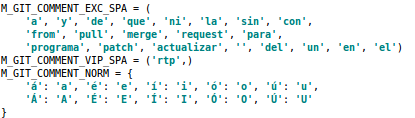
\includegraphics[width=16cm]{img/Selection_028_git_comentarios}
   \caption{Parámetros para la extracción de significantes de comentarios de \textit{commits}}
   \label{figura:git_commnet}
\end{figure}

Toda la información extraída según cada funcionalidad, se proporciona estructurada y los \textit{commits} relacionados entre sí para que pueda ser todo almacenado en BBDD.


\subsubsection{Módulo de análisis de código Python} 
\label{subsec:mod_anal_python}

En el análisis de los elementos del código fuente, introducimos en el diseño las funcionalidades que aportan la librería estándar \textit{Ast} y la librería externa \textit{Astor}, cuya función es la de procesar árboles de gramática abstracta, en Python.


Con ellas, podemos recuperar todos los elementos de código y sus propiedades en una estructura de árbol. Para la funcionalidad de este módulo, ambas librerias nos simplifican la implementación y abre nuevas posibilidades a futuras automatizaciones de Misture. \textit{Astor} nos proporciona algunas capacidades adicionales para manipular estos árboles y convertir el árbol a otras estructuras, incluyendo su impresión a texto de nodos de código.


Esta funcionalidad la añadimos al módulo \textit{PyGrammarAnaly}, para extraer datos por módulo sobre sus clases, métodos, línea y nombre, y pueda volcarse en la colección \textbf{UdFuente}. No obstante, mantenemos la anterior funcionalidad de la clase \textit{PyModuleCont} y la trasladamos a este módulo, para su uso en prácticas pequeñas o sobre versiones antiguas de Python.


\subsubsection{Módulo de análisis de estilo y calidad de código} 
\label{subsec:mod_anal_codigo}

En la implementación se mantuvo en gran medida la funcionalidad del módulo \textit{CodeAnaly}. Se sustituyeron las llamadas a las utilidades por sus librerías equivalentes en Python. Se consiguió una pequeña mejora en la extracción de la información de Pylint obteniendo la salida de los errores en JSON.


La principal novedad, es la introducción de una nueva utilidad de análisis de \textit{Flake8}, que combina, el análisis de estilo de \textit{Pep8} con el análisis estático de \textit{Pyflakes}, similar a \textit{Pylint}. Asimismo, permite la instalación de otros plugins para ampliar el análisis. Por lo que extendemos, con los paquetes \textit{McCabe} y \textit{Hackings}, aumentando la cantidad de comprobaciones y códigos de error disponibles.


\subsubsection{Módulos de análisis de XML y trazas Wireshark}
\label{subsec:mod_anal_xml_wireshark}

En el análisis de los \textit{scripts} semiautomáticos de las experiencias piloto, comentamos que existía un análisis de ficheros XML, que consistía en implementar un pequeño parser SAX específico para la corrección que comprueba la validación deseada sobre los elementos XML.


En esta versión,  se ha empezado a introducir una aproximación mediante análisis del árbol DOM, con ayuda de la librería Beautiful Soup 4, que genera dicho árbol y nos proporciona un potente conjunto de funciones para navegar.


Gracias a esto, hemos implementado un pequeño analizador dedicado a PDML que obtiene algunas estadísticas de las trazas. Como por ejemplo, para extraer la composición de tramas de los paquetes de una trama.

\begin{figure}[H]
   \centering
   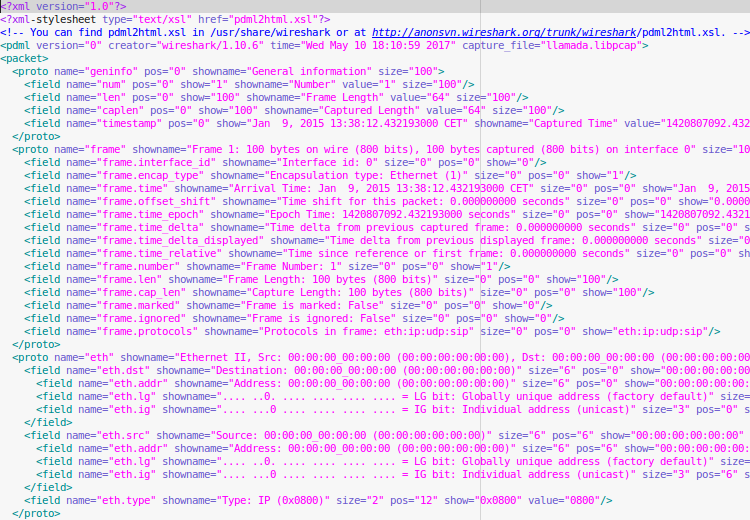
\includegraphics[width=15cm]{img/Selection_015_pdml_1}
   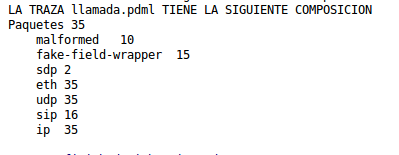
\includegraphics[width=8cm]{img/Selection_029_pdml}
   \caption{El PDML de la traza son elementos \textit{packet} con elementos \textit{proto} en su interior.}
   \label{figura:pdml}
\end{figure}


\newpage

\subsection{Generación de examen}

En el diseño, se incluye este módulo que permite la generación y carga para la corrección de cada alumno, de un conjunto de preguntas acerca del código y de los conceptos que el profesor quiera poner a prueba. Para ello, consideramos dos fuentes:

\begin{itemize}
\item Se carga un fichero JSON con las preguntas desde la ruta que se le indica como parámetro. La estructura de este JSON es una lista de objetos pregunta con los elementos enunciado, pregunta, tipo, opciones, resultados, etc.

\item A partir del análisis del código, se obtienen  algunos snippets del código de las fuentes Python, pertenecientes a correcciones de los diferentes alumnos de una misma actividad.
\end{itemize}


A partir de esas dos fuentes, y en función del tipo de pregunta, se rellenan documentos en la colección \textbf{CuestionExamen} de la BBDD para cada una de las correcciones. En el caso de las preguntas generadas a partir de snippets, se generan preguntas con opciones si o no sobre la autoría o sobre al nombre del fichero fuente al que pertenece.


Posteriormente, en caso de cargarse las respuestas en los documentos de \textbf{CuestionExamen}, podemos validarlas contra la respuesta esperada.


\section{Aplicación examen Django}

Una aplicación de examen recoge información a través de la base de datos MongoDB de Misture con la carga de las preguntas generadas.


Para los alumnos cuyos logines se encuentran en el conjunto de correcciones de la actividad, se activa la opción de contestar a las preguntas en forma de formularios Esta queda marcada como respondida una vez se pulse al botón de confirmación y queda asimismo registrado el momento en que fue contestada.


\section{Diseño de BBDD} 
\label{sec:bbdd}
En la versión más reciente de Misture, se optó por emplear el sistema de base de datos MongoDB, con bases de datos no relacionales, sin esquema, o mejor dicho, de esquema dinámico.\\


La elección de MongoDB para almacenar todos los datos obtenidos de los análisis de los repositorios, pruebas, y comprobaciones de código, en principio facilita y nos permite ser más ágiles durante el desarrollo y prueba de los diferentes módulos y funcionalidades. Por una parte por no trabajar con un esquema rígido y por otra porque MongoDB encaja muy bien con los tipos de datos nativos de Python – objetos, listas, diccionarios-.\\


Adicionalmente, se buscó os una librería ODM -Object Document Mapper- para MongoDB en Python, que permitiera operar con la BBDD como si fuera un objeto, facilitando aún más nuestra labor. En un primer momento se eligió \textit{Mongoengine}, aunque al final en Misture se utilizó \textit{PyMODM}.\\


Se debe recordar, que la estructura y validaciones de los campos definidos en las clases documento del ODM que representan los documentos de las colecciones de MongoDB son transparentes al propio MongoDB, se producen en el lado de la aplicación a través del ODM.\\

A continuación, vamos a enumerar los diferentes documentos considerados para poder llevar a cabo la funcionalidad básica de Misture.\\


\newpage	%TODO AJUSTE

\begin{figure}[H]
   \centering
   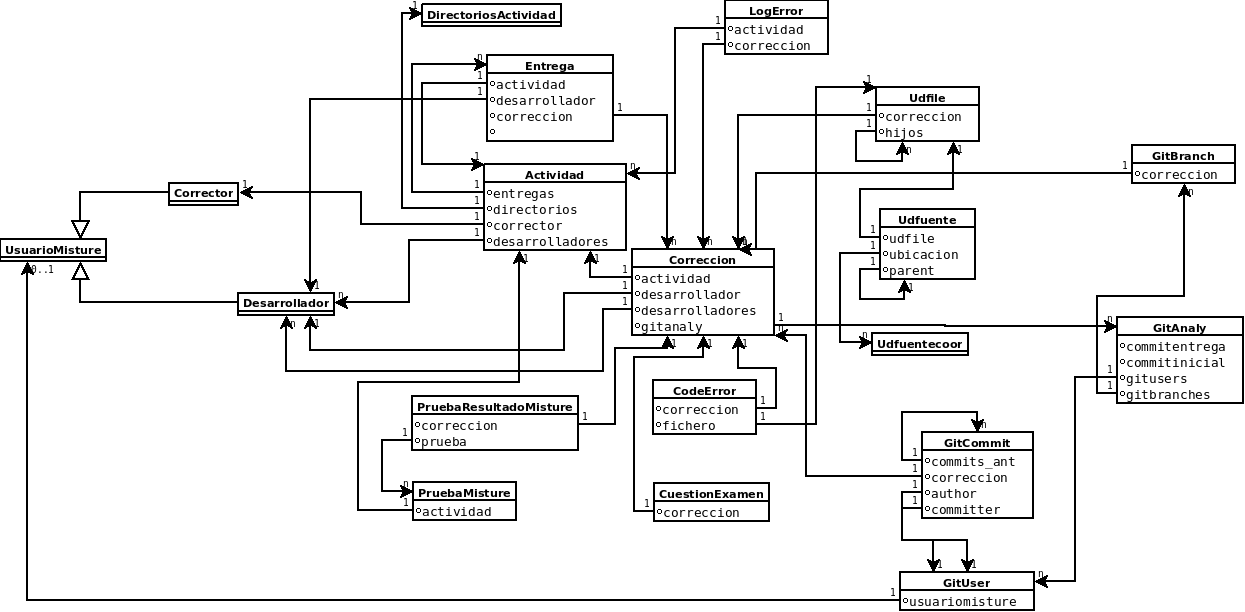
\includegraphics[width=16cm]{img/Diagram4_bbdd}
   \caption{Representación de BBDD incluida en Misture}
   \label{figura:bbdd}
\end{figure}

\vspace{3cm}



\begin{description}
\item \textbf{LogError} es la clase del documento donde se vuelcan los errores controlados de la ejecución de Misture.
\begin{itemize}
\item descripcion
\item accion
\item traza
\item fecha
\item actividad: referencia a \textbf{Actividad}
\item correccion: referencia a \textbf{Correccion}
\end{itemize}
\item \textbf{UsuarioMisture} representa a un usuario del sistema Misture.
\begin{itemize}
\item login
\item email
\item rol
\item date
\end{itemize}
\item \textbf{Corrector} es la clase heredera de \textbf{UsuarioMisture} que modela las particularidades del usuario corrector.
\begin{itemize}
\item actividades: referencia a \textbf{Actividad}
\item rol
\item superrol
\end{itemize}
\item \textbf{Desarrollador} es la subclasde de \textbf{UsuarioMisture} que representa al desarrollador.
\begin{itemize}
\item emails
\item rol
\end{itemize}
\item \textbf{}

\item \textbf{DirectoriosActividad} representan las rutas particulares donde se ubicarían los ficheros de la actividad a corregir.
\begin{itemize}
\item pbase
\item pentrega
\item presultados
\item perrores
\item ptest
\item ppruebas
\end{itemize}
\item \textbf{Actividad} es la clase que representa una actividad, con sus datos básicos para ser corregida.
\begin{itemize}
\item descripcion
\item corrector: referencia a \textbf{Corrector}
\item desarrolladores: referencia a \textbf{Desarrollador}
\item entregas: documento Entrega
\item directorios: documento \textbf{DirectoriosActividad}
\item ficheros\_entrega
\end{itemize}
\item \textbf{Correccion} es la clase que representa a la ejecución de una corrección de una entrega de un alumno.
\begin{itemize}
\item fecha
\item actividad: referencia a \textbf{Actividad}
\item desarrollador: referencia a \textbf{Desarrollador}
\item desarrolladores: referencia a \textbf{Desarrollador}
\item gitanaly: documento \textbf{GitAnaly}
\end{itemize}
\item \textbf{Entrega} es la clase que modela los elementos necesarios para emprender la corrección de la actividad de un alumno particular.
\begin{itemize}
\item actividad: referencia a \textbf{Actividad}
\item desarrollador: referencia a \textbf{Desarrollador}
\item modo
\item ubicacion
\item correccion: referencia al documento corrección.
\end{itemize}
\item \textbf{Udfile} representa a un fichero o directorio de una entrega.
\begin{itemize}
\item correccion: referencia a \textbf{Correccion}
\item pathrel
\item nombre
\item tipo
\item hijos: referencia a \textbf{Udfile}
\item lenguaje
\item sloc
\end{itemize}
\item \textbf{Udfuente} representa a un elemento de código dentro de un fichero fuente.
\begin{itemize}
\item udfile: referencia a Udfile
\item parent: referencia a Udfuente
\item nombre
\item ubicacion: documento Udfuentecoor
\item snippet
\end{itemize}
\item \textbf{Udfuentecoor} es la clase que modela la ubicación del elemento de código dentro de una fuente.
\begin{itemize}
\item filaini
\item filafin
\item col
\item pos
\end{itemize}

\item \textbf{}
\item \textbf{CodeError}: modela un error de estilo
\begin{itemize}
\item correccion: referencia a \textbf{Correccion}
\item fichero
\item fila
\item columna
\item tipo
\item codigo
\item descripcion
\end{itemize}
\item \textbf{GitUser}: usuario \textit{committer} o \textit{author} de Git.
\begin{itemize}
\item  name
\item email
\end{itemize}
\item \textbf{GitBranch}: datos de una rama de un repositorio Git de una corrección concreta.
\begin{itemize}
\item correccion: referencia a \textbf{Correccion}
\item nombre
\item nombre\_remote
\item targetid
\end{itemize}
\item \textbf{GitCommit}: representa un commit
\begin{itemize}
\item correccion: referencia a \textbf{Correccion}
\item idhex
\item orden
\item author: referencia a \textbf{GitUser}
\item committer: referencia a \textbf{GitUser}
\item time
\item offset
\item mensaje
\item palabrasclave
\item commits\_ant: referencia a \textbf{GitCommit}
\item ficheros
\end{itemize}
\item \textbf{GitAnaly} es la clase que contienen los datos de analisis de un repositorio Git.
\begin{itemize}
\item commitentrega: referencia a \textbf{GitCommit}
\item commitinicial: referencia a \textbf{GitCommit}
\item numcommits
\item palabras
\item intervalos
\item gitusers: referencia a \textbf{GitUser}
\item gitbranches: referencia a \textbf{GitBranch}
\end{itemize}
\item \textbf{PruebaMisture} representa la definición de una prueba de caja negra.
\begin{itemize}
\item actividad: referencia a \textbf{Actividad}.
\item titulo
\item descripcion
\item comando
\item salida
\end{itemize}
\item \textbf{PruebaResultadoMisture} representa el resultado de una ejecución de prueba sobre una corrección de una entrega particular.
\begin{itemize}
\item correccion: referencia a \textbf{Corrección}.
\item prueba: referencia a \textbf{PruebaMisture}
\item tipo\_salida
\item path\_salida
\item espruebavalida
\end{itemize}
\item \textbf{CuestionExamen} representa las preguntas del examen
\begin{itemize}
\item correccion: referencia a \textbf{Corrección}
\item tipo\_pregunta
\item contenido\_pregunta
\item tipo\_respuesta
\item opciones\_respuesta
\item opciones\_validas
\item respondida
\item respuesta
\item fecha\_respuesta
\end{itemize}
\end{description}